\documentclass[11pt]{article}
\usepackage[margin=1in]{geometry}
\usepackage{amsmath,amssymb}
\usepackage{enumitem}
\usepackage{booktabs}
\usepackage{tikz}
\usetikzlibrary{positioning,arrows.meta}

\newcommand{\indep}{{\bot\negthickspace\negthickspace\bot}}
\DeclareMathOperator{\E}{\mathbb{E}}

\pagestyle{plain}

\begin{document}

\begin{center}
{\Large \textbf{Statistics 256: Causality}} \\[6pt]
{\large In-class Activity 5: Selection on Observables --- Identification}
\end{center}

\vspace{4pt}
\noindent\textbf{Name(s):} \hrulefill

\vspace{14pt}

%%% QUESTION 1 %%%
\noindent\textbf{Question 1: Positivity in the wild}

A researcher estimating the effect of a job-training program on earnings conditions on $X = (\text{age}, \text{gender}, \text{prior-earnings quartile})$.  

\begin{enumerate}[label=(\roman*)]
\item Would we believe CI here? Why or why not?
\vspace{2cm}

\item In the cell $\{\text{age 55+, male, top quartile}\}$ there are 0 treated units (though several control units). What problem does this cause? 

\vspace{1.5cm}

\item List one or two things you could do to address the last problem. 

\vspace{2cm}

\end{enumerate}


%%% QUESTION 2 %%%
\noindent\textbf{Question 2: Seeing CI on the graph}

\medskip
\noindent Consider the following DAG.  $X$ is observed; $D$ is treatment; $Y$ is the outcome.

\begin{center}
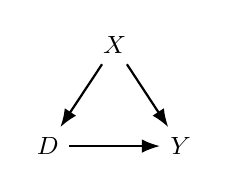
\begin{tikzpicture}[->,>=Latex,thick,node distance=1.6cm,
  every node/.style={font=\small}]
\node (X) {$X$};
\node (D) [below left= 0.8cm and 0.3cm of X] {$D$};
\node (Y) [below right=0.8cm and 0.3cm of X] {$Y$};
\draw (X) -- (D);
\draw (X) -- (Y);
\draw (D) -- (Y);
\end{tikzpicture}
\end{center}

\begin{enumerate}[label=(\alph*)]
\item Draw $G_{\underline{D}}$ (the test graph: delete all arrows out of $D$; relabel the outcome as $Y_d$). How can you use this to argue for conditionaly ignorability on the graph? (What test do you do; what is the CI statement you are looking to support?).

\clearpage

\item Draw the SWIG under $do(D=d)$ (split the $D$ node as $D \mid d$; descendants of $D$ become subscripted).  Using d-separation in the SWIG, can you support CI? 

\vspace{3.0cm}

\item Now suppose there is \emph{also} an unobserved variable $U$ that causes both $D$ and $Y$.  Using either the test-graph or SWIG, see if conditioning on $X$ alone still gives CI? 

\vspace{2.5cm}
\end{enumerate}

\medskip

%%% QUESTION 3 %%%
\noindent\textbf{Question 3: A job-training study}

\medskip
\noindent A program ($D$) may affect earnings ($Y$).  You have pre-treatment data on age, education, and average earnings over the prior 5 years.

\begin{enumerate}[label=(\alph*)]
\item Assuming $X = (\text{age}, \text{education}, \text{prior earnings})$ blocks all backdoor paths from $D$ to $Y$, write conditional ignorability in PO notation using this $X$.

\vspace{2cm}

\item Give an example of an \textit{unobserved} variable that would plausibly violate CI.  (Hint: what might affect both program participation and earnings but is not in $X$?)

\vspace{2cm}

\item Suppose a colleague adds ``whether the participant found a job within 3 months of program start'' to $X$.  Is this going to help or hurt, and why?

\vspace{1.1cm}
\end{enumerate}

\end{document}
